% Introduction
\chapter{Introduction}

\begin{figure}
    \begin{center}
        \input{node_modules/@faaas/perf-v8-event-loop-results/assets/faas-profile-waiting-on-io.pgf}
    \end{center}
    \caption{\faas{} function execution profile}
\end{figure}

\faasxlong{} provides an abstraction over application development, decomposing programs into isolated stateless units called `functions', invoked by events such as HTTP requests, or messages received from a message bus\cite{ibmWhatFaaSFunctionasaService2024}.

This abstraction simplifies development, allowing developers to focus on the underlying business logic of their system, rather than managing and scaling infrastructure. Typically, developers design serverless functions to be stateless\cite{ggailey777AzureFunctionsBest2022}, enabling horizontal scaling\cite{ngoEvaluatingScalabilityElasticity2022}, communicating with persistent storage to persist state between function invocations.

In these execution environments, whilst `functions' are running, they are allocated, guaranteed and billed for resources such as CPU and memory throughout the lifecycle of its invocation. Whilst in theory this seems beneficial, in practice, this leads to wasted resources, as the function may be awaiting an asynchronous operation to complete, such as a network request.

In these environments, `functions' are typically implemented either as containers or as virtual machines running atop a serverless `runtime'; whilst these containers are awaiting I/O such as network requests, resources are still allocated, used to determine whether execution can continue.

This research aims to yield control back to the runtime from these `functions' whilst awaiting asynchronous operations to complete, allowing useful work to be scheduled by the runtime. Throughout this report, we propose three main contributions:

\begin{itemize}
    \item The \faaasc{} compiler that performs code splitting of JavaScript serverless functions, allowing a function to optionally be deployed in a split manner on any supported Serverless\cite{serverlessServerlessZeroFrictionServerless2024} platform.

    \item The \faaastime{} serverless runtime stack that accurately bills, composes and executes serverless JavaScript functions emitted by \faaasc{}.

    \item A costing analysis and evaluation of the required advancements to the serverless ecosystem to provide cost reductions by carrying out code splitting.
\end{itemize}

\section{Motivation}
% Syscall Calls Breakdown
\begin{figure}
    \begin{center}
        \input{node_modules/@faaas/perf-v8-event-loop-results/assets/faas-profile-strace-calls.pgf}
    \end{center}
    \caption{\faas{} petstore syscall calls profile}
\end{figure}

% Syscall Time Breakdown
\begin{figure}
    \begin{center}
        \input{node_modules/@faaas/perf-v8-event-loop-results/assets/faas-profile-strace-time.pgf}
    \end{center}
    \caption{\faas{} petstore syscall time profile}
\end{figure}

\faaslong{} has become increasingly more common amongst system architectures since the introduction of AWS Lambda\cite{amazonAWSLambda2024}. Typical \faas{} workloads can be characterised as `glue', most commonly handling HTTP requests and interacting with a form of persistent storage --- in fact, around 50\% of all serverless functions fall into this category\cite{eismannReviewServerlessUse2020}.

\faas{} architectures generally tend to decrease costs, achieving this by using a fine-grained billing model as described in Section \ref{sec:faas-billing-models}, charging per invocation, and for compute and memory allocations in subsecond increments over the duration of execution, ensuring wasted resources are released back to the cloud provider once a function terminates.

The resolution of the billing model however extends only to the level of granularity of functions, whereby resources are allocated for the entire lifetime of the function's execution. This is particularly important when considering that serverless suffers from additional latency when accessing persistent storage, for example, the average latency between AWS Lambda and DynamoDB is usually between \qtyrange{60}{90}{\ms}\cite{ghoshCachingTechniquesImprove2020}.

% PProf Sample from PetStore PutPet Function
\begin{figure*}
    \begin{center}
        \begin{tikzpicture}[scale = 0.75, every node/.style={scale=0.75}]
            \input{node_modules/@faaas/perf-v8-event-loop-results-pprof/assets/faas-profile-pprof-put-pet.pgf}
        \end{tikzpicture}
    \end{center}
    \caption{\faas{} petstore PutPet pprof sample}
\end{figure*}

Since the median execution time for serverless functions lies between milliseconds and a second\cite{eismannReviewServerlessUse2020}, this latency accounts for a significant proportion of time when resources are allocated and unused during function execution time. Developers are charged for this time, and cannot temporarily yield resources back to the host until the asynchronous action completes. This is refered to as the double billing problem\cite{baldiniServerlessTrilemmaFunction2017,yuCharacterizingServerlessPlatforms2020} and discussed further in Section \ref{sec:double-billing-problem}.

\begin{figure}[t]
    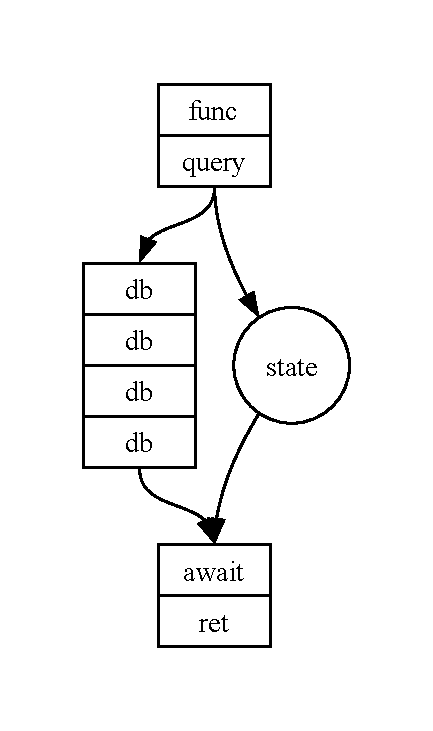
\includegraphics[width=\linewidth]{node_modules/@faaas/double-billing-problem/assets/double-billed-db-split.pdf}
    \caption{Illustration of termination function execution once DB request has been sent, with DB responsible for invoking the remaineder of the function with the result of the query.}
    \label{fig:double-billing-db-split}
\end{figure}
